Source reconstruction refers to the localisation of the electrical activity of the brain. In the case of this thesis, we are referring to EEG source localization, which is also called the reverse problem. Electrical activity within the brain is measured on the scalp using EEG electrodes. This is the forward problem. The reverse problem maps the measurements from the EEG electrodes back into the brain. \cite{schoffelen2009source}

\section{Reverse Problem}

Figure~\ref{source-local-img} visualizes the reverse problem. This is an ill-posed problem. EEG electrodes measure the scalp, in effect measuring a 2D grid. However, the brain is a 3D object. This means that information is inherently lost when EEG is used. One of the consequences is there are many different solutions to the reverse problem. 

\begin{figure}[!htb]
\caption{EEG Source Localisation \cite{source-loc-img}.}
\label{source-local-img}
    \centering
    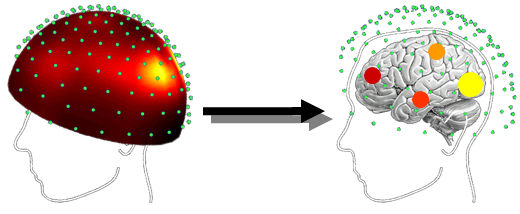
\includegraphics[width=\textwidth]{fig/source_recon}
\end{figure}

Equation~\ref{reverse} represents source localisation. $X$ represents the scalp recorded EEG activity. $S$ represents the electrical sources within the brain, a current density vector. $L$ represents the head volume conductor model. The reverse problem is about finding $S$, this is represented in equation~\ref{reverse2}.

\begin{equation}\label{reverse}
X = LS + n
\end{equation}

\begin{equation}\label{reverse2}
O(S) = min||X - LS||^2 
\end{equation}

\section{Head Volume Conductor Model}

Several different head volume conductor models can be used. The two most popular are the simple head models and the realistic head models. Simple head models model the brain as a single sphere with a couple layers. This model also assumes a uniform medium within the brain. Using a simple head model is fast and simple. However, it is not accurate. 

The realistic head model is an accurate model, but it is computationally much more expensive. Different techniques are used to construct a head model such as finite element or finite boundary techniques. 

\section{Dipoles}

The electrical activity from neural populations can be represented as a dipole. The inverse problem is essentially about determining the location, orientation, amplitude and number of these dipoles

There are practical limits to the number of dipoles that can be used. One of the most important limits is the spatial resolution of EEG. EEG can only measure electrical activity with a certain accuracy. This is due to the fact that the electrical activity is measured on the scalp, and each electrode records a linear combination of the underlying neural sources. This happens due to the low conductivity of the layers that are separating the cortex from the surface of the scalp (such as the skull, skin, and cerebrospinal fluid). The phenomena of how different mixtures of sources reach the scalp, how they attenuate and spread through the different layers of the head is referred to as volume conduction. We will elaborate on this further in the thesis.

\section{Algorithms}\label{source-alg}

There are different kind of algorithms used to solve the inverse problem. There is dipole fitting, which involves only a small number of dipoles. The locations, orientations, and magnitudes of these dipoles needs to be calculated. For some experiments, this method can be good enough, since a single dipole can account for 80\% of all electrical activity \cite{cohen2014analyzing}. Dipole fitting can be performed by a number of different software programs or matlab toolboxes, including BESA, eeglab and fieldtrip \cite{hoechstetter2004besa, delorme2004eeglab, oostenveld2011fieldtrip}.

Then there are nonadaptive distributed-source imaging methods and adaptive distributed-source imaging methods. The idea of distributed-source imaging is that thousands of dipoles are placed within the brain on fixed locations with fixed orientations. This leaves only the magnitude to be computed. This is done by assigning electrode weights to each dipole.

Nonadaptive methods compute these electrode weights based on the electrode locations. This means that the weights are fixed over time and frequency. sLORETA is a commonly used nonadaptive inverse-source imaging technique \cite{pascual2002standardized}. The provided data used in this thesis has also been source-reconstructed using sLORETA. Other nonadaptive methods include LORETA and minimum-norm estimator \cite{pascual1994low, hamalainen1994interpreting}.

Nonadaptive methods are relatively fast to compute, are applicable to single time points and their result looks like FMRI activation maps. However, there are also some disadvantages. One issue is the number of comparisons that need to be computed in statistical analyses. In the case of 10,000 dipoles over time and frequency with two experiment conditions, there over more than 100 million possible statistical comparisons that need to be computed. \cite{cohen2014analyzing}

Adaptive distributed-source imaging have a different way of computing the electrode weights. The recorded data is also used to compute the weights. The weights are not fixed over time and frequency. The accuracy of adaptive methods is often quite high, but they are much more complicated with many more parameters to be set. Beamforming is a class of algorithms that is most commonly used adaptive distributed-source imaging method \cite{gross2001dynamic, van1997localization}. 

\section{Practical Limits}

Within a simulated environment, high spatial localization accuracy can be obtained. However, in practive, there are many issues. There are always uncertainties regarding electrode positions, brain anatomy, head movement and scalp conductivity. This means that spatial accuracy is often a few centimeters in size. The smallest voxels which are created by source reconstruction are typically 5-10 mm$^3$ in size. \cite{grech2008review} 

Without knowledge of the inverse problem, it might seem that source reconstruction is not a big deal. It might even seem to only bring advantages, since you can work within the actual cortical areas. However, source reconstruction comes with its fair share of problems and inaccuracies. 

Within the context of this thesis, knowledge of the inverse problem is essential. While the data was already source-reconstructed, for the reasons above, it is important to know the inverse problem. 